\documentclass[12pt]{article}

% ========== Paquetes ===========

% Codificación de caracteres e idioma
\usepackage[utf8]{inputenc}
\usepackage[spanish]{babel}

% Paquete para referencias bibliográficas
\usepackage[backend=biber, style=authoryear]{biblatex}

% Tamaño de página y márgenes
\usepackage[letterpaper, margin=2.54cm]{geometry}

% Comillas, columnas, gráficos, símbolos matemáticos e ingreso de código de programación
\usepackage{csquotes, multicol, graphicx, amssymb, amsmath, listings, xcolor}

% Uso de punto decimal, en lugar de coma
\decimalpoint

% Cambia el nombre de Listing a Código, lista de código
\renewcommand{\lstlistingname}{Código}

% Separación de columnas y sangría
% \setlength{\columnsep}{1cm} 
% \setlength{\parindent}{0cm}

% Páginado
\pagestyle{plain}

% Evitar separación de palabras
% \hyphenpenalty=10000
% \exhyphenpenalty=10000
% \sloppy

% Archivo de referencias bibliográficas
\addbibresource{bib/referencias.bib}

% Estilos de color en código de programación
\definecolor{codegreen}{rgb}{0,0.6,0}
\definecolor{codegray}{rgb}{0.5,0.5,0.5}
\definecolor{codepurple}{rgb}{0.58,0,0.82}
\definecolor{backcolour}{rgb}{0.95,0.95,0.92}
\lstdefinestyle{mystyle}{
    backgroundcolor=\color{backcolour},   
    commentstyle=\color{codegreen},
    keywordstyle=\color{magenta},
    numberstyle=\tiny\color{codegray},
    stringstyle=\color{codepurple},
    basicstyle=\ttfamily\footnotesize,
    breakatwhitespace=false,         
    breaklines=true,                 
    captionpos=b,                    
    keepspaces=true,                 
    numbers=left,                    
    numbersep=5pt,                  
    showspaces=false,                
    showstringspaces=false,
    showtabs=false,                  
    tabsize=2
}
\lstset{style=mystyle}

% ========== Documento ==========

\begin{document}

% ========== Portada ============
\begin{titlepage}
	\centering
	{\scshape\LARGE Universidad Aztlán \par}
	\vspace{1cm}
	{\scshape\Large Campus Playa del Carmen \par}
	\vspace{1.75cm}
	{\scshape\Huge Organizar, representar e interpretar conjuntos de datos mediante herramientas de estadística descriptiva para apoyar la toma de decisiones \par}
    \vfill
    {\itshape\Large Actividades \par}
	\vspace{2cm}
    {\itshape\Large Realizado por: \par}
    {\Large Fernando Ángel Trejo Germán \par}
	{\Large José Rosendo Camal Teh \par}
	\vfill
	{\Large Ingeniería en Sistemas Computacionales \par}
	{\Large Tercer Cuatrimestre \par}
	{\Large Probabilidad y Estadística \par}
	\vfill
	{\Large Profe. José Noé Pool Ay \par}
	\vfill
	{\Large 01 de agosto de 2026 \par}
	\vfill
	{\Large Playa del Carmen, Quintana Roo \par}
\end{titlepage}

\tableofcontents
\listoffigures
\listoftables
\lstlistoflistings
\newpage

% ========== Cuerpo =============

% Introducción 
\section*{\centering Introducción}
\addcontentsline{toc}{section}{Introducción}

La estadística descriptiva permite organizar, representar e interpretar datos para comprender la información que tenemos a la mano y por consecuencia, impacta en la manera de tomar decisiones. Las técnicas y conceptos de esta disciplina contribuyen a que usemos los datos que tenemos a disposición, que los interpretemos de la mejor manera. Varios conceptos como media, mediana, moda, media agrupada, mediana agrupada, moda agrupada, varianza y desviación estándar, varianza agrupada, desviación estándar agrupada dejan de ser meras nociones matemáticas y se convierten en instrumentos para la interpretación de información basada en datos que junto con los histogramas y tablas, nos ayudan a comprender la relevancia de la estadística descriptiva. Igualmente, si consideramos que el uso de lenguajes de programación puede ayudar a la automatización de los procesos mecánicos, esto da como resultado la agilización y facilita la labor de la interpretación de datos. Todo esto nos prepara mejor para el mundo profesional actual y futuro.

\newpage

% Desarrollo
\section*{\centering Actividades}
\addcontentsline{toc}{section}{Actividades}

\textbf{Instrucciones:} El desarrollo de estos ejercicios contribuirá a comprender la importancia de la estadística en diferentes áreas del conocimiento, ya que facilita la interpretación de datos y apoya la toma de decisiones basada en evidencia, tanto en el ámbito académico como en situaciones de la vida cotidiana.

%\begin{multicols}{2}
%\end{multicols}

% Actividad 1
\subsection*{\centering Conceptos básicos}
\addcontentsline{toc}{subsection}{Conceptos básicos}
\textbf{Ejercicio 1:} Clasifica las siguientes variables como cualitativas nominales, cualitativas ordinales, cuantitativas discretas o cuantitativas continuas.

\begin{itemize}
    \item [a.] Edad de una persona.
    \item [b.] Color de ojos.
    \item [c.] Número de hijos.
    \item [d.] Nivel de satisfacción (Bajo, Medio, Alto).
    \item [e.] Estatura.
\end{itemize}

\paragraph{\textbf{Solución: }}
Los incisos \textbf{a} y \textbf{c} son variables de tipo \textit{cuantitativa discreta}. El inciso \textbf{b} es una variable \textit{cualitativa nominal}. Por otro lado, el inciso \textbf{d} es una variable \textit{cualitativa ordinal}. Por último, el inciso \textbf{e} es una variable \textit{cuantitativa continua}.

% Actividad 2
\subsection*{\centering Descripción de datos}
\addcontentsline{toc}{subsection}{Descripción de datos}
\textbf{Ejercicio 2:} Una tienda registró las ventas diarias durante una semana: 

\[15, 18, 12, 20, 16, 22, 17.\]

Determina:
\begin{itemize}
    \item [] Valor máximo.
    \item [] Valor mínimo.
    \item [] Rango.
\end{itemize}

Ordena los datos de menor a mayor.

\paragraph{\textbf{Solución: }}

Primero ordenamos los números de las ventas diarias de menor a mayor y queda así: $12, 15, 16, 17, 18, 20, 22$. Posteriormente, tomamos el número $12$ como el \textbf{valor mínimo} porque es el número más pequeño del listado, del mismo modo, agarramos el número $22$ como \textbf{valor máximo} ya que es el número mayor de las ventas diarias. Como paso siguiente, calculamos el \textbf{rango} restando al valor máximo el valor mínimo dejando el resultado de $10$.

De manera adicional, realizamos un script en lenguaje de programación \textit{Python} para resolver la tarea mecánica de arriba y así fortalecer nuestras habilidades de codificación y de matemáticas.
\lstinputlisting[language=Python, caption=Descripción de datos]{py/descripcion_datos.py}

El \textit{output} del programa es: \\
    
    \indent \verb|Ventas diarias: [15, 18, 12, 20, 16, 22, 17]| \\
    \indent \verb|Valor maximo: 22| \\
    \indent \verb|Valor minimo: 12| \\
    \indent \verb|Rango: 10| \\
    \indent \verb|Valores ordenados: [12, 15, 16, 17, 18, 20, 22]| \\


% Actividad 3
\subsection*{\centering Medidas de tendencia central y dispersión}
\addcontentsline{toc}{subsection}{Medidas de tendencia central y dispersión}
\textbf{Ejercicio 3:} Las calificaciones de 10 estudiantes fueron:
\[70, 75, 80, 85, 90, 85, 80, 95, 100, 80\]

Calcula:
\begin{itemize}
    \item Media.
    \item Mediana.
    \item Moda.
    \item Rango.
    \item Varianza.
    \item Desviación estándar.
\end{itemize}

\paragraph{\textbf{Solución: }}

La \textbf{media} de las calificaciones es $84$. Esta se obtiene con la fórmula:
\[\textit{Media} = {\textit{suma de todos los datos} \over \textit{número de datos}}\]

La \textbf{mediana} es $82.5$ y este es el valor central de las calificaciones. Se obtiene de dos formas, si el número de datos es impar es el valor que queda a la mitad cuando se ordenan los datos de menor a mayor o viceversa. Cuando la cantidad de datos es par se aplica la siguiente fórmula considerando los dos valores centrales:
\[\textit{Mediana} = {{{\textit{valor central inferior} + \textit{valor central superior}}} \over 2}\]

La \textbf{moda} es el número $80$ ya que se repite más veces, unas 3 veces, y no hay otro número que tenga una cantidad igual o mayor de repeticiones. Esta se encuentra contando las ocurrencias y la que tenga mayor frecuencia se elige como la moda.

El \textbf{rango} es $30$ y es la diferencia entre el número máximo (100) y el número mínimo (70). Se calcula así $\textit{Rango} = x_{max} - x_{min}$ o se puede interpretar así:
\[\textit{Rango} = \text{max(\textit{conjunto de datos A}}) - min(\textit{conjunto de datos A})\]

La \textbf{varianza} es $74$ y se calculó con la expresión para varianza poblacional, donde la media poblacional es la media aritmética de todas las calificaciones:
\[\sigma^2 = {\sum{(\textit{dato individual} - \textit{media poblacional})^2} \over \textit{cantidad de datos total}}\]

La \textbf{desviación estándar} es $8.6$ y es la raíz cuadrada de la varianza previamente calculada. La expresión simplificada de la desviación estándar es:
\[\sigma = \sqrt{\sigma^2}\]

De manera adicional, realizamos un script en lenguaje de programación \textit{Python} para automatizar los cálculos y así fortalecer nuestras habilidades de codificación y de matemáticas.
\lstinputlisting[language=Python, caption=Tendencia central y dispersión]{py/tendencia_central_dispersion.py}

El \textit{output} del programa es:
\begin{verbatim}
Media: 84.0
Mediana: 82.5
Rango: 30
Varianza: 74.0
Desviacion estandar: 8.6
Conteo para obtener moda: {80:3, 85:2, 100:1, 70:1, 75:1, 90:1, 95:1}
\end{verbatim}

% Actividad 4
\subsection*{\centering Parámetros para datos agrupados}
\addcontentsline{toc}{subsection}{Parámetros para datos agrupados}
\textbf{Ejercicio 4:} La siguiente tabla representa las edades de un grupo de personas.

\begin{table}[h!]
    \begin{center}
        \begin{tabular}{|c|c|}
            \hline
            Intervalo & Frecuencia \\
            \hline
            10-19 & 5 \\
            20-29 & 8 \\
            30-39 & 12 \\
            40-49 & 10 \\
            50-59 & 5 \\
            \hline
        \end{tabular}
    \end{center}
\end{table}

Calcula:
\begin{itemize}
    \item Media agrupada.
    \item Mediana agrupada.
    \item Moda agrupada.
\end{itemize}

\paragraph{\textbf{Solución: }}

La \textbf{media agrupada} es $35.0$, la \textbf{mediana agrupada} es $35.83$ y la \textbf{moda agrupada} es $36.67$. 

La \textit{media agrupada} se obtiene con la fórmula:
\[\bar{x} = {{\sum{f_i \cdot m_i}} \over n}\]
Donde la media agrupada se representa como $\bar{x}$, las frecuencias (los valores individuales que tenemos en cada intervalo) de cada clase o intervalo se identifican como $f_i$, la suma de todas las frecuencias con $n$. La marca de clase es $m_i$ y se obtiene con el promedio de los límites superior e inferior por cada intervalo (o clase). La \textit{marca de clase} se calcula con:
\[Marca\ de\ clase = {{\text{límite superior} + \text{límite inferior}} \over 2}\]

La \textit{mediana agrupada} se obtiene con la siguiente fórmula:
\[Mediana\ agrupada = L_i + \left({{(n/2) - F_{ant}} \over f_{Me}}\right) \cdot c\]
Donde $L_i$ es el límite inferior de la clase mediana, $n$ es el total de datos, $F_{ant}$ es la frecuencia acumulada anterior a la clase mediana, $f_{Me}$ es la frecuencia de la clase mediana y $c$ es la amplitud de las clases. El \textit{límite inferior de la clase mediana} se obtiene identificando la primera clase cuya frecuencia acumulada supera $n/2$. Para encontrarla, sumamos las frecuencias de cada clase de arriba hacia abajo hasta superar dicho valor. La primera clase $10\text{-}19$ tiene una frecuencia de $5$, que aún no supera $n/2 = 20$. La segunda clase $20\text{-}29$ suma $8$ frecuencias más, dando una frecuencia acumulada de $13$, que tampoco supera $20$. La tercera clase $30\text{-}39$ suma $12$ frecuencias más, dando una frecuencia acumulada de $25$, que sí supera $20$. Por lo tanto, la clase mediana es $30\text{-}39$. Una vez identificada la clase, sustituimos en la fórmula: el límite inferior $L_i$ es $30$, la frecuencia acumulada anterior $F_{ant}$ es $13$, la frecuencia de la clase mediana $f_{Me}$ es $12$ y la amplitud $c$ es $10$. Al realizar la operación: $30 + ((20 - 13)/12) \cdot 10 = 35.83$.

La \textit{moda agrupada} es $36.67$ y corresponde al intervalo con mayor frecuencia, que es $30\text{-}39$ con $12$ datos. La moda agrupada se obtiene con la siguiente fórmula:
\[Moda\ agrupada = L_i + \left({\Delta_1 \over \Delta_1 + \Delta_2}\right) \cdot c\]
Donde $L_i$ es el límite inferior de la clase modal, $\Delta_1$ es la diferencia entre la frecuencia de la clase modal y la frecuencia de la clase anterior, $\Delta_2$ es la diferencia entre la frecuencia de la clase modal y la frecuencia de la clase siguiente y $c$ es la amplitud de las clases. La clase modal se identifica como la que tiene mayor frecuencia, en este caso $30\text{-}39$ con $12$ datos. Para calcular $\Delta_1$, restamos la frecuencia de la clase anterior ($20\text{-}29$, frecuencia $8$) a la frecuencia de la clase modal: $12 - 8 = 4$. Para calcular $\Delta_2$, restamos la frecuencia de la clase siguiente ($40\text{-}49$, frecuencia $10$) a la frecuencia de la clase modal: $12 - 10 = 2$. Sustituyendo los valores en la fórmula: $30 + (4/(4+2)) \cdot 10 = 36.67$.

De manera adicional, realizamos un script en lenguaje de programación \textit{Python} para automatizar los cálculos y así fortalecer nuestras habilidades de codificación y de matemáticas.
\lstinputlisting[language=Python, caption=Parámetros para datos agrupados]{py/parametros_datos_agrupados.py}

El \textit{output} del programa es:
\begin{verbatim}
Media agrupada: 35.0
Mediana agrupada: 35.83
Moda agrupada: 36.67
\end{verbatim}

% Actividad 5
\subsection*{\centering Distribución de frecuencias}
\addcontentsline{toc}{subsection}{Distribución de frecuencias}
\textbf{Ejercicio 5:} Con los siguientes datos:

\[12, 15, 18, 20, 15, 17, 18, 16, 19, 20, 18, 17, 16, 15, 18.\]

Construye una tabla con:
\begin{itemize}
    \item Frecuencia absoluta.
    \item Frecuencia acumulada.
    \item Frecuencia relativa.
    \item Frecuencia relativa acumulada.
\end{itemize}

\textbf{Solución: }

\begin{table}[h!]
    \begin{center}
        \begin{tabular}{|l|l|l|l|l|}
            \hline
            Dato & Frec. absoluta & Frec. acumulada & Frec. relativa & Frec. relativa acum. \\
            \hline
            12 & 1 & 1 & 0.07 (7\%) & 0.07 (7\%) \\
            15 & 3 & 4 & 0.20 (20\%) & 0.27 (27\%) \\
            16 & 2 & 6 & 0.13 (13\%) & 0.40 (40\%) \\
            17 & 2 & 8 & 0.13 (13\%) & 0.53 (53\%) \\
            18 & 4 & 12 & 0.27 (27\%) & 0.80 (80\%) \\
            19 & 1 & 13 & 0.07 (7\%) & 0.87 (87\%) \\
            20 & 2 & 15 & 0.13 (13\%) & 1.00 (100\%) \\
            \hline
        \end{tabular}
        \caption{Distribución de frecuencias}
        \label{tab:tabla_frecuencias}
    \end{center}
\end{table}

Primero ordenamos los datos de menor a mayor para facilitar el conteo: 12, 15, 15, 15, 16, 16, 17, 17, 18, 18, 18, 18, 19, 20, 20. Observamos que hay 7 valores distintos: $12, 15, 16, 17, 18, 19$ y $20$, con un total de $n = 15$ datos.

La \textbf{frecuencia absoluta} ($f_{abs}$) es el número de veces que aparece cada valor en el conjunto de datos. Se obtiene contando las ocurrencias de cada número: el $12$ aparece $1$ vez, el $15$ aparece $3$ veces, el $16$ aparece $2$ veces, el $17$ aparece $2$ veces, el $18$ aparece $4$ veces, el $19$ aparece $1$ vez y el $20$ aparece $2$ veces. Como paso siguiente, verificamos que la suma de todas las frecuencias absolutas sea igual al total de datos: $1 + 3 + 2 + 2 + 4 + 1 + 2 = 15$, lo cual coincide con $n$.

La \textbf{frecuencia acumulada} se obtiene sumando las frecuencias absolutas de manera progresiva desde el valor más pequeño hasta el más grande. Comenzamos con el $12$ que tiene frecuencia $1$, luego sumamos la frecuencia del $15$ ($3$) quedando $1 + 3 = 4$, después sumamos la del $16$ ($2$) quedando $4 + 2 = 6$, y así sucesivamente hasta llegar al último valor $20$ cuya frecuencia acumulada debe ser igual a $n = 15$.

La \textbf{frecuencia relativa} indica la proporción de datos que corresponden a cada valor. Se calcula dividiendo la frecuencia absoluta de cada número entre el total de datos: $\frac{f_{abs}}{n}$
Por ejemplo, para el $15$ la frecuencia relativa es $3/15 = 0.20$, lo que significa que el $20\%$ de los datos son iguales a $15$. Las frecuencias relativas de todos los valores deben sumar $1$.

La \textbf{frecuencia relativa acumulada} se obtiene de forma similar a la frecuencia acumulada, pero sumando las frecuencias relativas de manera progresiva. Comenzamos con la frecuencia relativa del $12$ ($0.07$), le sumamos la del $15$ ($0.20$) quedando $0.27$, y continuamos hasta llegar al último valor $20$ cuya frecuencia relativa acumulada debe ser igual a $1$.

De manera adicional, realizamos un script en lenguaje de programación \textit{Python} para automatizar los cálculos y así fortalecer nuestras habilidades de codificación y de matemáticas.
\lstinputlisting[language=Python, caption=Frecuencias]{py/frecuencias.py}

El \textit{output} de nuestro script es:
\begin{verbatim}
=======================================================================
|    Numero   |   F. abs.   |F. abs. acum.|   F. rel.   |F. rel. acum.|
=======================================================================
|      12     |      1      |      1      |     0.07    |     0.07    |
|      15     |      3      |      4      |     0.2     |     0.27    |
|      16     |      2      |      6      |     0.13    |     0.4     |
|      17     |      2      |      8      |     0.13    |     0.53    |
|      18     |      4      |      12     |     0.27    |     0.8     |
|      19     |      1      |      13     |     0.07    |     0.87    |
|      20     |      2      |      15     |     0.13    |     1.0     |
=======================================================================
\end{verbatim}

% Actividad 6
\subsection*{\centering Técnicas de agrupación}
\addcontentsline{toc}{subsection}{Técnicas de agrupación}
\textbf{Ejercicio 6:} Las estaturas (cm) de 20 estudiantes son:

\[155, 158, 160, 162, 164, 165, 166, 167, 168, 170,\]
\[171, 172, 173, 174, 175, 176, 178, 180, 182, 185.\]

Agrupa los datos en 5 clases e indica:
\begin{itemize}
    \item Amplitud de clase.
    \item Límites de cada intervalo.
    \item Frecuencia de cada clase.
\end{itemize}

\textbf{Solución: }

\begin{table}[h!]
    \begin{center}
        \begin{tabular}{|l|l|}
            \hline
            Límite de intervalo & Frecuencia \\
            \hline
            {[}155-161) & 3 \\
            {[}161-167) & 4 \\
            {[}167-173) & 5 \\
            {[}173-179) & 5 \\
            {[}179-185{]} & 3 \\
            \hline
        \end{tabular}
        \caption{Intervalos y su frecuencia}
        \label{tab:tabla_clases}
    \end{center}
\end{table}

Para agrupar los datos en 5 clases, primero calculamos el \textbf{rango} restando el valor mínimo al valor máximo: $185 - 155 = 30$. Posteriormente, obtenemos la \textbf{amplitud de clase} dividiendo el rango entre el número de clases: $30/5 = 6$. Una vez tenemos la amplitud, partimos desde el valor mínimo ($155$) e incrementamos de $6$ en $6$ para obtener los límites de cada intervalo: la primera clase comienza en $155$ y termina en $155 + 6 = 161$, la segunda comienza en $161$ y termina en $161 + 6 = 167$, y así hasta completar las 5 clases. Las primeras cuatro clases son \textit{intervalos semiabiertos}, es decir, incluyen el límite inferior pero excluyen el límite superior. La última clase es un \textit{intervalo cerrado}, lo que significa que incluye ambos límites, inferior y superior, para asegurar que el valor máximo ($185$) quede comprendido dentro de la agrupación.

Para obtener la \textbf{frecuencia de cada clase}, contamos cuántos datos caen en cada intervalo. La primera clase $[155\text{-}161)$ contiene los valores $155, 158$ y $160$, dando una frecuencia de $3$. La segunda clase $[161\text{-}167)$ contiene $162, 164, 165$ y $166$, dando una frecuencia de $4$. La tercera clase $[167\text{-}173)$ contiene $167, 168, 170, 171$ y $172$, dando una frecuencia de $5$. La cuarta clase $[173\text{-}179)$ contiene $173, 174, 175, 176$ y $178$, dando una frecuencia de $5$. La última clase $[179\text{-}185]$ contiene $180, 182$ y $185$, dando una frecuencia de $3$. Verificamos que la suma de todas las frecuencias sea igual al total de datos: $3 + 4 + 5 + 5 + 3 = 20$, lo cual coincide con la cantidad de mediciones de estaturas de 20 alumnos.

De manera adicional, realizamos un script en lenguaje de programación \textit{Python} para automatizar los cálculos y así fortalecer nuestras habilidades de codificación y de matemáticas.
\lstinputlisting[language=Python, caption=Límites de clase y su frecuencia]{py/tecnicas_agrupacion.py}

El \textit{output} de nuestro script es:
\begin{verbatim}
Amplitud de clase: 6.0
=================================
| Limites de clase | Frecuencia |
=================================
|    [155-161)     |     3      |
|    [161-167)     |     4      |
|    [167-173)     |     5      |
|    [173-179)     |     5      |
|    [179-185]     |     3      |
=================================
\end{verbatim}

% Actividad 7
\subsection*{\centering Técnicas de muestreo}
\addcontentsline{toc}{subsection}{Técnicas de muestreo}
\textbf{Ejercicio 7:} Una universidad tiene 2000 estudiantes. Indica qué técnica de muestreo utilizarías en cada caso:
\begin{itemize}
    \item [a.] Elegir estudiantes al azar usando una lista.
    \item [b.] Elegir únicamente estudiantes de Ingeniería y Medicina.
    \item [c.] Seleccionar un salón completo al azar.
    \item [d.] Elegir cada estudiante número 20 de la lista.
\end{itemize}

Identifica el tipo de muestreo.

\paragraph{\textbf{Solución: }}

El inciso \textbf{a} realizaríamos un \textit{muestreo aleatorio simple}. En el inciso \textbf{b} realizaríamos un \textit{muestreo estratificado} ya que los estudiantes de Ingeniería y Medicina son grupos específicos de la población estudiantil. En el inciso \textbf{c} sería un \textit{muestreo por conglomerados} ya que se selecciona un salón completo al azar, el cual es un grupo natural de la población. Mientras, para el inciso \textbf{d} sería un \textit{muestreo sistemático} ya que se va a elegir de forma aleatoria, pero con una base fija (la elección del número 20 de cada salón).

% Actividad 8
\subsection*{\centering Histogramas}
\addcontentsline{toc}{subsection}{Histogramas}
\textbf{Ejercicio 8:} Las edades de 18 personas son:

\[18, 19, 20, 20, 21, 21, 22, 22, 22, 23, 24, 24, 25, 25, 26, 27, 28, 29.\]

Construye:
\begin{itemize}
    \item La tabla de frecuencias.
    \item El histograma correspondiente.
\end{itemize}

\textbf{Solución: }

\begin{table}[h!]
    \begin{center}
        \begin{tabular}{|l|l|l|l|l|}
            \hline
            Edad & F. absoluta & F. abs. acumulada & F. relativa & F. rel. acumulada \\
            \hline
            18 & 1 &  1 & 0.06 (6\%) & 0.06 (6\%) \\
            19 & 1 &  2 & 0.06 (6\%) & 0.11 (11\%) \\
            20 & 2 &  4 & 0.11 (11\%) & 0.22 (22\%) \\
            21 & 2 &  6 & 0.11 (11\%) & 0.33 (33\%) \\
            22 & 3 &  9 & 0.17 (17\%) & 0.50 (50\%) \\
            23 & 1 & 10 & 0.06 (6\%) & 0.56 (56\%) \\
            24 & 2 & 12 & 0.11 (11\%) & 0.67 (67\%) \\
            25 & 2 & 14 & 0.11 (11\%) & 0.78 (78\%) \\
            26 & 1 & 15 & 0.06 (6\%) & 0.83 (83\%) \\
            27 & 1 & 16 & 0.06 (6\%) & 0.89 (89\%) \\
            28 & 1 & 17 & 0.06 (6\%) & 0.94 (94\%) \\
            29 & 1 & 18 & 0.06 (6\%) & 1.00 (100\%) \\
            \hline
        \end{tabular}
        \caption{Tabla de edades y sus frecuencias}
        \label{tab:tabla_edades}
    \end{center}
\end{table}

Para construir la tabla de frecuencias, primero ordenamos los datos de menor a mayor: $18, 19, 20, 20, 21, 21, 22, 22, 22, 23, 24, 24, 25, 25, 26, 27, 28, 29$. Observamos que hay 12 valores distintos, con un total de $n = 18$ datos. La \textbf{frecuencia absoluta} se obtiene contando las ocurrencias de cada edad: $18$ aparece $1$ vez, $19$ aparece $1$ vez, $20$ aparece $2$ veces, $21$ aparece $2$ veces, $22$ aparece $3$ veces, $23$ aparece $1$ vez, $24$ aparece $2$ veces, $25$ aparece $2$ veces, y las edades $26, 27, 28$ y $29$ aparecen $1$ vez cada una. Verificamos que la suma de las frecuencias absolutas sea igual al total de datos: $1 + 1 + 2 + 2 + 3 + 1 + 2 + 2 + 1 + 1 + 1 + 1 = 18$, lo cual coincide con el total de $n$.

La \textbf{frecuencia acumulada} se obtiene sumando las frecuencias absolutas de manera progresiva desde la edad más pequeña hasta la más grande, comenzando con $1$ para los $18$ años y llegando a $18$ en los $29$ años. La \textbf{frecuencia relativa} indica la proporción de datos que corresponden a cada edad y se calcula dividiendo la frecuencia absoluta entre el total de datos. Por ejemplo, para los $22$ años la frecuencia relativa es $3/18 = 0.17$, lo que significa que el $17\%$ de las personas tienen $22$ años. La \textbf{frecuencia relativa acumulada} se obtiene sumando las frecuencias relativas de manera progresiva hasta llegar a $1$.

\begin{figure}[htb!]
	\centering
	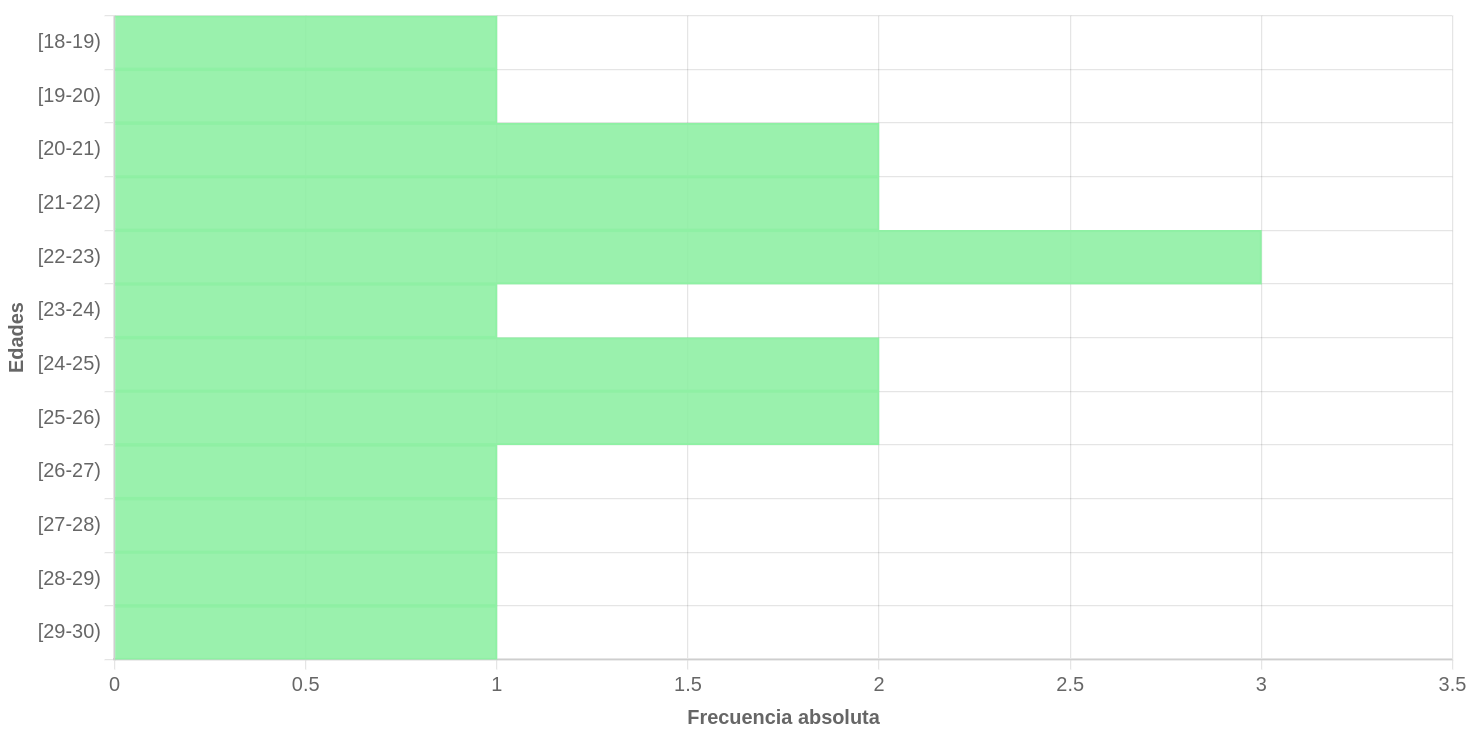
\includegraphics[width=0.9\linewidth]{img/histogramas.png}
	\caption{Histograma de edades}
\end{figure}

De manera adicional, realizamos un script en lenguaje de programación \textit{Python} para automatizar los cálculos y así fortalecer nuestras habilidades de codificación y de matemáticas.
\lstinputlisting[language=Python, caption=Frecuencias e histograma]{py/histogramas.py}

El \textit{output} de nuestro script es:
\begin{verbatim}
=======================================================================
|    Numero   |   F. abs.   |F. abs. acum.|   F. rel.   |F. rel. acum.|
=======================================================================
|      18     |      1      |      1      |     0.06    |     0.06    |
|      19     |      1      |      2      |     0.06    |     0.11    |
|      20     |      2      |      4      |     0.11    |     0.22    |
|      21     |      2      |      6      |     0.11    |     0.33    |
|      22     |      3      |      9      |     0.17    |     0.5     |
|      23     |      1      |      10     |     0.06    |     0.56    |
|      24     |      2      |      12     |     0.11    |     0.67    |
|      25     |      2      |      14     |     0.11    |     0.78    |
|      26     |      1      |      15     |     0.06    |     0.83    |
|      27     |      1      |      16     |     0.06    |     0.89    |
|      28     |      1      |      17     |     0.06    |     0.94    |
|      29     |      1      |      18     |     0.06    |     1.0     |
=======================================================================
=================================
|     Frecuencias absolutas     |
=================================
| 18 | ======               | 1 |
| 19 | ======               | 1 |
| 20 | =============        | 2 |
| 21 | =============        | 2 |
| 22 | ==================== | 3 |
| 23 | ======               | 1 |
| 24 | =============        | 2 |
| 25 | =============        | 2 |
| 26 | ======               | 1 |
| 27 | ======               | 1 |
| 28 | ======               | 1 |
| 29 | ======               | 1 |
=================================
\end{verbatim}


% Actividad 9
\subsection*{\centering Ejercicio integrador}
\addcontentsline{toc}{subsection}{Ejercicio integrador}
\textbf{Ejercicio 9:} Los tiempos (minutos) empleados por 15 trabajadores para completar una tarea fueron:

\[18, 20, 19, 22, 21, 23, 24, 20, 19, 21, 22, 23, 25, 24, 20.\]

Realiza lo siguiente:
\begin{itemize}
    \item Ordena los datos.
    \item Calcula media, mediana y moda.
    \item Calcula la desviación estándar.
    \item Construye la distribución de frecuencias.
    \item Dibuja el histograma.
\end{itemize}

\paragraph{\textbf{Solución: }}

Primero ordenamos los tiempos en minutos de los trabajadores de menor a mayor: 18, 19, 19, 20, 20, 20, 21, 21, 22, 22, 23, 23, 24, 24, 25, con un total de $n = 15$ datos (igual a la cantidad de 15 empleados).

La \textbf{media} es $21.4$ y se obtiene sumando todos los tiempos y dividiendo entre el número de datos. La suma de los tiempos es $18 + 19 + 19 + 20 + 20 + 20 + 21 + 21 + 22 + 22 + 23 + 23 + 24 + 24 + 25 = 321$, por lo que la media es $321/15 = 21.4$.

La \textbf{mediana} es $21$ y es el valor central de los datos ordenados. Como $n$ es impar ($15$), el valor central corresponde a la octava posición, que es $21$. De lo contrario, si $n$ fuera par, la mediana se obtendría promediando los dos valores centrales con la fórmula:
\[Mediana = {{valor\ central\ inferior + valor\ central\ superior} \over 2}\]

La \textbf{moda} es $20$ ya que aparece $3$ veces, más que cualquier otro valor. Adicionalmente, los valores $19, 21, 22, 23$ y $24$ aparecen $2$ veces cada uno, por lo que no pueden considerarse como moda ya que $2 < 3$.


La \textbf{desviación estándar} es $2.03$ y es la raíz cuadrada de la varianza:
\[\sigma = \sqrt{\sigma^2}\]
La varianza (en este caso) se calcula con la expresión para \textit{varianza poblacional}, donde la \textit{media poblacional} es la media de todos los tiempos registrados:
\[\sigma^2 = {\sum{(\textit{dato individual} - \textit{media poblacional})^2} \over \textit{cantidad de datos total}}\]

Sustituyendo con los datos de tiempo, donde la $media = 21.4$, $n = 15$ y una vez calculadas las diferencias elevadas al cuadrado:
\begin{align*}
\sigma^2 &= \frac{11.56 + 11.52 + 5.88 + 0.32 + 0.72 + 5.12 + 13.52 + 12.96}{15} \\
&= \frac{61.6}{15} \\
&= 4.11 \\
\sigma &= \sqrt{4.11}  \\
&= 2.03
\end{align*}

Para la distribución de frecuencias, contamos las ocurrencias de cada tiempo. La \textbf{frecuencia absoluta} es el número de veces que aparece cada valor en el conjunto de datos registrado.

La \textbf{frecuencia acumulada} se obtiene sumando las frecuencias absolutas de manera progresiva desde el valor más pequeño hasta el más grande, comenzando con $1$ para los $18$ minutos y llegando a $15$ en los $25$ minutos.

La \textbf{frecuencia relativa} indica la proporción de datos que corresponden a cada tiempo y se calcula dividiendo la frecuencia absoluta entre el total de datos ($f_{abs}/n$). Por ejemplo, para los $20$ minutos la frecuencia relativa es $3/15 = 0.20$, lo que significa que el $20\%$ de los trabajadores tardaron $20$ minutos.

La \textbf{frecuencia relativa acumulada} se obtiene sumando las frecuencias relativas de manera progresiva, comenzando con $0.07$ para los $18$ minutos y llegando a $1$ en los $25$ minutos, lo que indica que el $100\%$ de los datos están comprendidos en el rango de $18$ a $25$ minutos.

\begin{table}[h!]
    \begin{center}
        \begin{tabular}{|l|l|l|l|l|}
            \hline
            Tiempo (min) & F. absoluta & F. abs. acumulada & F. relativa & F. rel. acumulada \\
            \hline
            18 & 1 &  1 & 0.07 (7\%) & 0.07 (7\%) \\
            19 & 2 &  3 & 0.13 (13\%) & 0.20 (20\%) \\
            20 & 3 &  6 & 0.20 (20\%) & 0.40 (40\%) \\
            21 & 2 &  8 & 0.13 (13\%) & 0.53 (53\%) \\
            22 & 2 & 10 & 0.13 (13\%) & 0.67 (67\%) \\
            23 & 2 & 12 & 0.13 (13\%) & 0.80 (80\%) \\
            24 & 2 & 14 & 0.13 (13\%) & 0.93 (93\%) \\
            25 & 1 & 15 & 0.07 (7\%) & 1.00 (100\%) \\
            \hline
        \end{tabular}
        \caption{Tiempos de tarea y sus frecuencias}
        \label{tab:tabla_tiempos}
    \end{center}
\end{table}

\begin{figure}[htb]
	\centering
	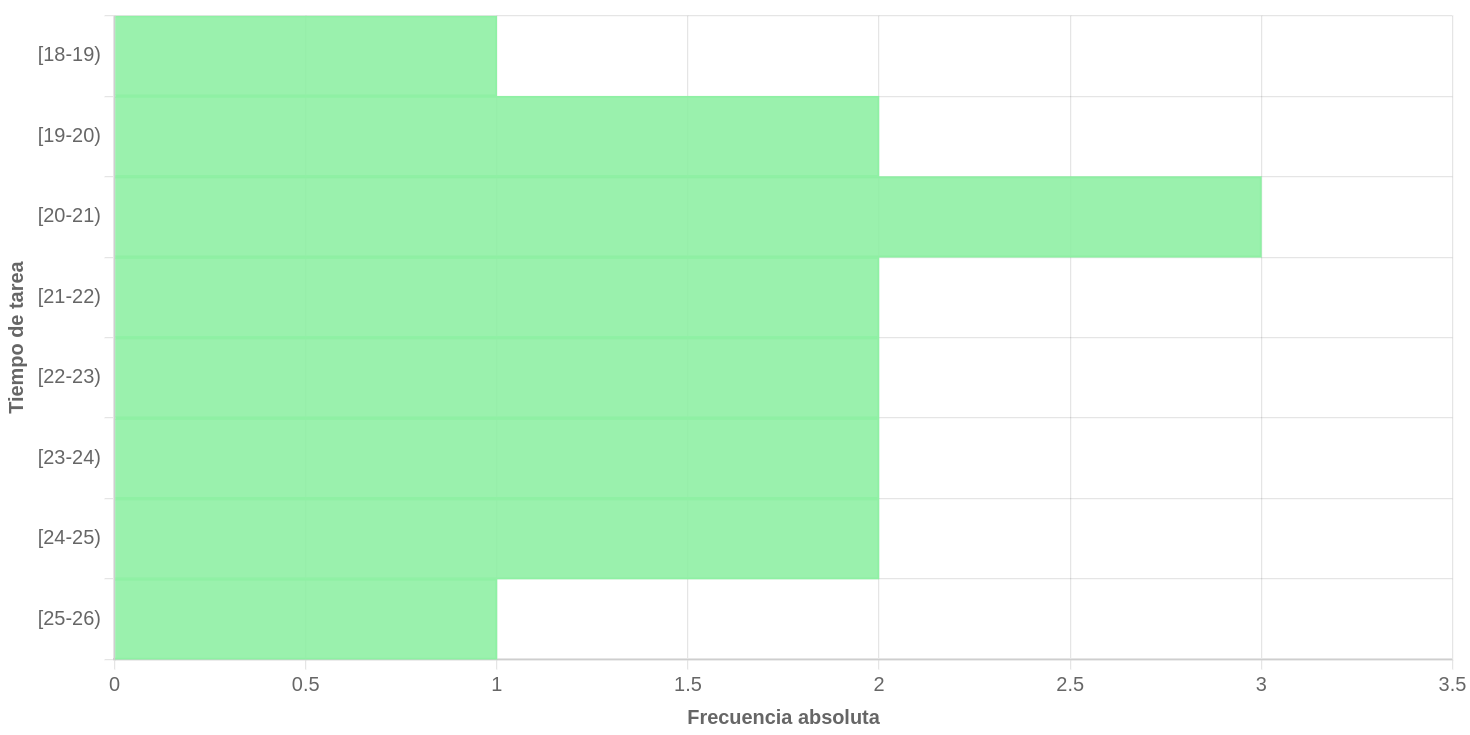
\includegraphics[width=0.9\linewidth]{img/ejercicio_integrador.png}
	\caption{Histograma de tiempo de tareas}
\end{figure}
\newpage

De manera adicional, realizamos un script en lenguaje de programación \textit{Python} para automatizar los cálculos y así fortalecer nuestras habilidades de codificación y de matemáticas.
\lstinputlisting[language=Python, caption=Tendencia central-Dispersión y Frecuencias e Histograma]{py/ejercicio_integrador.py}

El \textit{output} de nuestro script es:
\begin{verbatim}
Datos ordenados: [18, 19, 19, 20, 20, 20, 21, 21, 22, 22, 23, 23, 24, 24, 25]
Media: 21.4
Mediana: 21
Desviacion estandar: 2.03
Conteo para obtener moda: {20:3, 19:2, 21:2, 22:2, 23:2, 24:2, 18:1, 25:1}
=======================================================================
|    Numero   |   F. abs.   |F. abs. acum.|   F. rel.   |F. rel. acum.|
=======================================================================
|      18     |      1      |      1      |     0.07    |     0.07    |
|      19     |      2      |      3      |     0.13    |     0.2     |
|      20     |      3      |      6      |     0.2     |     0.4     |
|      21     |      2      |      8      |     0.13    |     0.53    |
|      22     |      2      |      10     |     0.13    |     0.67    |
|      23     |      2      |      12     |     0.13    |     0.8     |
|      24     |      2      |      14     |     0.13    |     0.93    |
|      25     |      1      |      15     |     0.07    |     1.0     |
=======================================================================
=================================
|     Frecuencias absolutas     |
=================================
| 18 | ======               | 1 |
| 19 | =============        | 2 |
| 20 | ==================== | 3 |
| 21 | =============        | 2 |
| 22 | =============        | 2 |
| 23 | =============        | 2 |
| 24 | =============        | 2 |
| 25 | ======               | 1 |
=================================
\end{verbatim}

% Actividad 10
\subsection*{\centering Problema de aplicación}
\addcontentsline{toc}{subsection}{Problema de aplicación}
\textbf{Ejercicio 10:} Una empresa registró el número de productos vendidos por 30 empleados en un día:

\[12, 15, 18, 20, 21, 19, 22, 25, 18, 17, 19, 20, 21, 23, 24, \]
\[18, 19, 20, 22, 24, 25, 26, 27, 28, 18, 19, 20, 21, 22, 23.\]

Realiza:
\begin{itemize}
    \item [1.] Construye la tabla de distribución de frecuencias.
    \item [2.] Agrupa los datos en intervalos.
    \item [3.] Calcula la media, mediana y moda.
    \item [4.] Calcula la varianza y la desviación estándar.
    \item [5.] Elabora un histograma.
    \item [6.] Interpreta los resultados obtenidos.
\end{itemize}

\paragraph{\textbf{Solución: }}

Primero ordenamos los 30 datos de menor a mayor y sacamos la frecuencia. La \textbf{frecuencia absoluta} indica cuántas veces aparece cada número de productos vendidos. Verificamos que la suma de las frecuencias absolutas sea igual al total de datos: $1 + 1 + 1 + 4 + 4 + 4 + 3 + 3 + 2 + 2 + 2 + 1 + 1 + 1 = 30$ y este número coincide con el total de empleados.

La \textbf{frecuencia acumulada} se obtiene sumando las frecuencias absolutas de manera progresiva desde el valor más pequeño hasta el más grande, comenzando con $1$ para los $12$ productos vendidos y llegando a $30$ en $28$ productos vendidos. La \textbf{frecuencia relativa} indica la proporción de datos que corresponden a cada valor y se calcula dividiendo la frecuencia absoluta entre el total de datos.

La \textbf{frecuencia relativa acumulada} se obtiene sumando las frecuencias relativas de manera progresiva hasta llegar a $1$.

\begin{table}[h!]
    \begin{center}
        \begin{tabular}{|l|l|l|l|l|}
            \hline
            Dato & F. absoluta & F. abs. acumulada & F. relativa & F. rel. acumulada \\
            \hline
            12 & 1 &  1 & 0.03 (3\%) & 0.03 (3\%) \\
            15 & 1 &  2 & 0.03 (3\%) & 0.07 (7\%) \\
            17 & 1 &  3 & 0.03 (3\%) & 0.10 (10\%) \\
            18 & 4 &  7 & 0.13 (13\%) & 0.23 (23\%) \\
            19 & 4 & 11 & 0.13 (13\%) & 0.37 (37\%) \\
            20 & 4 & 15 & 0.13 (13\%) & 0.50 (50\%) \\
            21 & 3 & 18 & 0.10 (10\%) & 0.60 (60\%) \\
            22 & 3 & 21 & 0.10 (10\%) & 0.70 (70\%) \\
            23 & 2 & 23 & 0.07 (7\%) & 0.77 (77\%) \\
            24 & 2 & 25 & 0.07 (7\%) & 0.83 (83\%) \\
            25 & 2 & 27 & 0.07 (7\%) & 0.90 (90\%) \\
            26 & 1 & 28 & 0.03 (3\%) & 0.93 (93\%) \\
            27 & 1 & 29 & 0.03 (3\%) & 0.97 (97\%) \\
            28 & 1 & 30 & 0.03 (3\%) & 1.00 (100\%) \\
            \hline
        \end{tabular}
        \caption{Ventas diarias y sus frecuencias}
        \label{tab:tabla_ventas}
    \end{center}
\end{table}

Para los intervalos, el rango es $16$ y el número de clases es $\sqrt{30} \approx 5.48 \approx 6$, por lo que la amplitud de clase es $16/6 \approx 2.67 \approx 3$, redondeando a $3$ se obtienen $6$ clases. Se parte desde el mínimo ($12$) y se incrementa de $3$ en $3$: $[12\text{-}15), [15\text{-}18), [18\text{-}21), [21\text{-}24), [24\text{-}27), [27\text{-}30]$. Para conseguir la frecuencia de cada clase, se cuenta cuántos datos caen en cada intervalo.

\begin{table}[h!]
    \begin{center}
        \begin{tabular}{|l|l|}
            \hline
            Intervalo & Frecuencia \\
            \hline
            {[}12-15) & 1 \\
            {[}15-18) & 2 \\
            {[}18-21) & 12 \\
            {[}21-24) & 8 \\
            {[}24-27) & 5 \\
            {[}27-30{]} & 2 \\
            \hline
        \end{tabular}
        \caption{Intervalos de ventas y su frecuencia}
        \label{tab:tabla_intervalos_ventas}
    \end{center}
\end{table}

Para calcular la \textbf{media agrupada}, se usa la fórmula:
\[\bar{x} = {{\sum{f_i \cdot m_i}} \over n}\]
Donde $\bar{x}$ es la media agrupada, $f_i$ es la frecuencia de cada clase, $m_i$ es la marca de clase y $n$ es el total de datos. La \textit{marca de clase} se obtiene con el promedio de los límites superior e inferior de cada intervalo:
\[Marca\ de\ clase = {{\text{límite superior} + \text{límite inferior}} \over 2}\]
Calculamos las marcas de clase: $13.5, 16.5, 19.5, 22.5, 25.5$ y $28.5$. Sustituyendo en la fórmula:
\[\bar{x} = {(1 \cdot 13.5 + 2 \cdot 16.5 + 12 \cdot 19.5 + 8 \cdot 22.5 + 5 \cdot 25.5 + 2 \cdot 28.5) \over 30} = {645 \over 30} = 21.5\]

La \textbf{mediana agrupada} se obtiene con la fórmula:
\[Mediana\ agrupada = L_i + \left({{(n/2) - F_{ant}} \over f_{Me}}\right) \cdot c\]
Donde $L_i$ es el límite inferior de la clase mediana, $F_{ant}$ es la frecuencia acumulada anterior a la clase mediana, $f_{Me}$ es la frecuencia de la clase mediana y $c$ es la amplitud de las clases. La clase mediana se identifica buscando la primera cuya frecuencia acumulada supera $n/2 = 15$, que es $[18\text{-}21)$. Sustituyendo con el límite inferior $L_i = 18$, la frecuencia acumulada anterior $F_{ant} = 3$, la frecuencia de la clase mediana $f_{Me} = 12$ y la amplitud $c = 3$: $18 + ((15 - 3)/12) \cdot 3 = 21.0$.

La \textbf{moda agrupada} corresponde al intervalo con mayor frecuencia, que es $[18\text{-}21)$ con $12$ datos. La \textit{clase modal} se obtiene identificando la clase con mayor frecuencia dentro de la distribución. Una vez identificada, la moda agrupada se calcula con:
\[Moda\ agrupada = L_i + \left({\Delta_1 \over \Delta_1 + \Delta_2}\right) \cdot c\]
Donde $L_i$ es el límite inferior de la clase modal, $\Delta_1$ es la diferencia entre la frecuencia de la clase modal y la de la anterior ($12 - 2 = 10$), $\Delta_2$ es la diferencia entre la frecuencia de la clase modal y la de la siguiente ($12 - 8 = 4$) y $c$ es la amplitud. Sustituyendo: $18 + (10/(10+4)) \cdot 3 = 20.14$.

Para calcular la \textbf{varianza} de los datos agrupados, se cuenta con la fórmula de varianza poblacional (para datos agrupados):
\[\sigma^2 = {\sum{\left[(\textit{frecuencia\ intervalo}) \cdot (\textit{marca de clase} - \textit{media agrupada})^2\right]} \over \textit{total de datos}}\]
La marca de clase se obtiene con el promedio de los límites de cada intervalo:
\[Marca\ de\ clase = {{\text{límite superior} + \text{límite inferior}} \over 2}\]
Sustituyendo con las marcas de clase ($13.5, 16.5, 19.5, 22.5, 25.5, 28.5$), las frecuencias y la media agrupada ($21.5$):
\begin{align*}
\sigma^2 &= \frac{1 \cdot (13.5 - 21.5)^2 + 2 \cdot (16.5 - 21.5)^2 + 12 \cdot (19.5 - 21.5)^2}{30} \\
&+ \frac{8 \cdot (22.5 - 21.5)^2 + 5 \cdot (25.5 - 21.5)^2 + 2 \cdot (28.5 - 21.5)^2}{30} \\
&= \frac{64 + 50 + 48 + 8 + 80 + 98}{30} = \frac{348}{30} = 11.6
\end{align*}

La \textbf{desviación estándar} es la raíz cuadrada de la varianza:
\[\sigma = \sqrt{\sigma^2} = \sqrt{11.6} = 3.41\]

\begin{figure}[htb!]
	\centering
	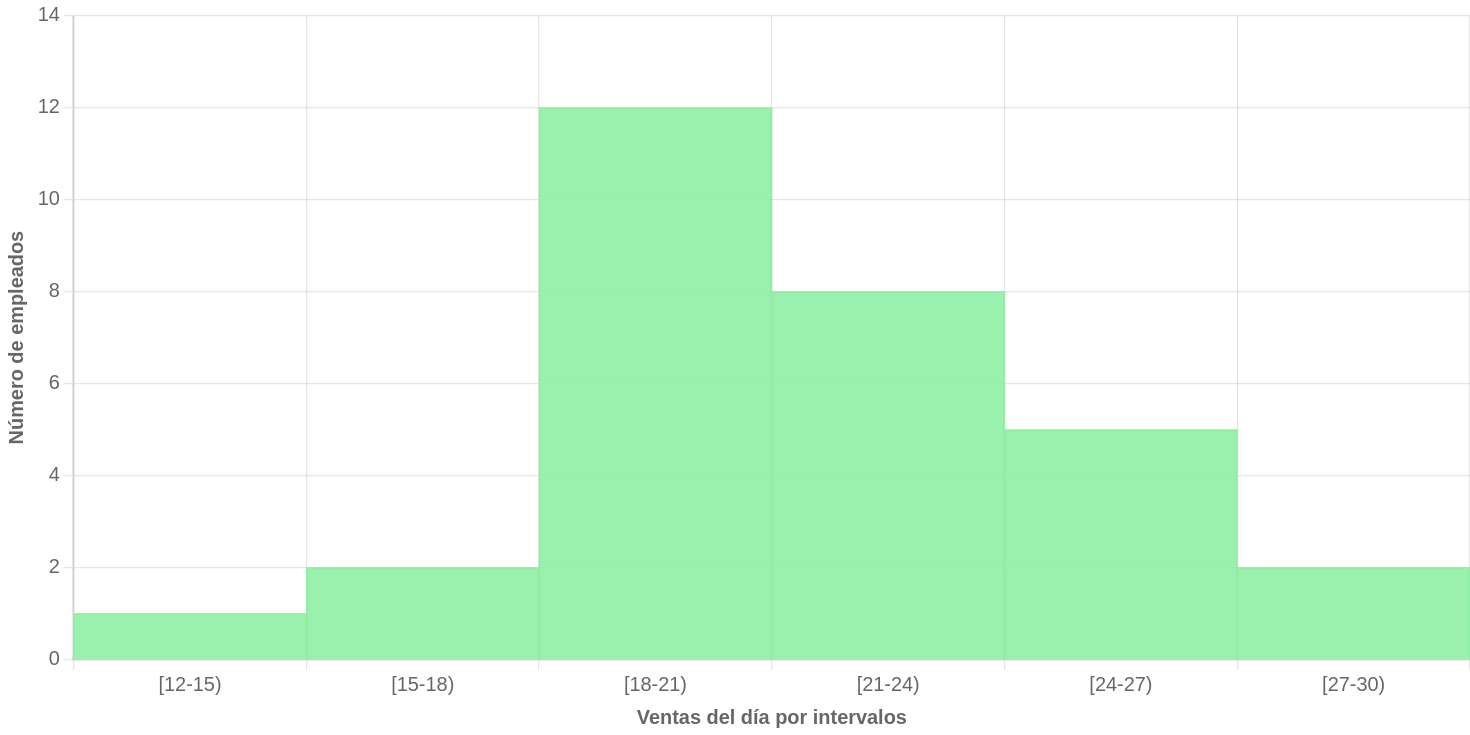
\includegraphics[width=0.9\linewidth]{img/problema_aplicacion.png}
	\caption{Ventas del día realizado por cada empleado}
\end{figure}

\textbf{Interpretación:} Los resultados indican que, en promedio, cada [grupo de] empleado[s] vendió alrededor de 21.5 productos en el día registrado. La mediana agrupada (21.0) y la moda agrupada (20.14) cercanas a la media sugieren que la distribución de ventas es bastante simétrica, es decir, no hay valores extremos que distorsionen el promedio. La desviación estándar agrupada de 3.41 productos indica que la mayoría de los empleados se encuentra dentro de un rango relativamente cercano a la media, entre aproximadamente 18 y 25 productos vendidos. Esto permite identificar que el rendimiento de los empleados es bastante uniforme, sin grandes diferencias entre los que menos vendieron (12 productos) y los que más vendieron (28 productos). En otras palabras, estamos viendo en el histograma una \textit{Campana de Gauss}.

De manera adicional, realizamos dos scripts en lenguaje de programación \textit{Python} para automatizar los cálculos y así fortalecer nuestras habilidades de codificación y de matemáticas. He aquí el primer programa:
\lstinputlisting[language=Python, caption=Amplitud con Límites de clase y Frecuencias]{py/problema_app_1.py}

El \textit{output} del primer script es:
\begin{verbatim}
=======================================================================
|    Numero   |   F. abs.   |F. abs. acum.|   F. rel.   |F. rel. acum.|
=======================================================================
|      12     |      1      |      1      |     0.03    |     0.03    |
|      15     |      1      |      2      |     0.03    |     0.07    |
|      17     |      1      |      3      |     0.03    |     0.1     |
|      18     |      4      |      7      |     0.13    |     0.23    |
|      19     |      4      |      11     |     0.13    |     0.37    |
|      20     |      4      |      15     |     0.13    |     0.5     |
|      21     |      3      |      18     |     0.1     |     0.6     |
|      22     |      3      |      21     |     0.1     |     0.7     |
|      23     |      2      |      23     |     0.07    |     0.77    |
|      24     |      2      |      25     |     0.07    |     0.83    |
|      25     |      2      |      27     |     0.07    |     0.9     |
|      26     |      1      |      28     |     0.03    |     0.93    |
|      27     |      1      |      29     |     0.03    |     0.97    |
|      28     |      1      |      30     |     0.03    |     1.0     |
=======================================================================

Amplitud de clase: 3.2
=================================
| Limites de clase | Frecuencia |
=================================
|     [12-15)      |     1      |
|     [15-18)      |     2      |
|     [18-21)      |     12     |
|     [21-24)      |     8      |
|     [24-27)      |     5      |
|     [27-30]      |     2      |
=================================
\end{verbatim}

He aquí el segundo programa:
\lstinputlisting[language=Python, caption=Tendencia central y Dispersión para datos agrupados]{py/problema_app_2.py}
Los resultados del segundo script son los siguientes:
\begin{verbatim}
Media agrupada: 21.5
Mediana agrupada: 21.0
Moda agrupada: 20.14
Varianza (usando frecuencias absolutas): 11.6
Desviacion estandar (usando frecuencias absolutas): 3.41
\end{verbatim}

\newpage

% Conclusión
\section*{\centering Conclusión}
\addcontentsline{toc}{section}{Conclusión}

El desarrollo de estas actividades nos permite comprender que la estadística descriptiva es una herramienta que siempre estamos usando, y cuyo valor puede ser tanto teórico como pragmático. Cada ejercicio propuesto nos ayuda a reconocer cómo se aplican los conceptos de media, mediana, moda, varianza, desviación estándar y histogramas en situaciones de la vida cotidiana y profesional, y cómo el uso de lenguajes de programación puede facilitar la interpretación de datos de manera más eficiente.

\newpage

% ========== Bibliografía =======

\nocite{*}
\printbibliography[heading=bibintoc]
\newpage

\end{document}